% This is an LPSC Abstract template for LaTeX 2e that is based off of the
% LaTeX article document class.

% $Id: lpsc_abstract.tex 11 2008-01-31 15:42:07Z rbeyer $

% Copyright (C) 2005,2007 Ross A. Beyer
% Copyright (C) 2008 Ross A. Beyer and Moses P. Milazzo
% Copyright (C) 2014 Moses P. Milazzo
%
% This work is licensed under the Creative Commons
% Attribution-Noncommercial-Share Alike 3.0 License. To view a copy
% of this license, visit http://creativecommons.org/licenses/by-nc-sa/3.0/;
% or, (b) send a letter to Creative Commons, 171 2nd Street, Suite
% 300, San Francisco, California, 94105, USA.

% Use the LaTeX article class.  Pass any options you like to article, except
% twocolumn.  We take care of that in the lpscabs pacakage below.
\documentclass[twoside]{article} 

\usepackage{times}				% Nice fonts, optional
\usepackage{hyperref}                % Needed for wrapping long URLs

\usepackage{graphicx}			% Nice graphics, optional

\usepackage[numbers]{natbib}	% Nice references, optional
\setlength{\bibsep}{0pt}		% Remove the spacing between bib entries
% These commands are relevant to natbib.  If you don't use
% natbib for your references, you should get rid of these, as well.
%\renewcommand{\bibfont}{\small}	% Change the font size of the bibliography
\renewcommand{\bibsection}{\subsubsection*{\hspace{0.5cm}References:}}
%								% Make the References heading smaller.

% To compress the section titles even more, use the titlesec package.
%\usepackage[small,compact]{titlesec}

\usepackage{paralist}			% For compressing bibliography into a paragraph

\usepackage{balance}			% For balancing columns on the page.
								
\usepackage{lpscabs}			% This is to take care of some LPSC abstract
								% document-specific things and set sizes.

\begin{document}

% The \titlearea command takes two arguments in curly braces {}.  The first
% will be used as the title, and the second as the author info.
% Use \\ \hrule here to put a horizontal rule across both columns

\titlearea{\LaTeX\ LPSC Abstract Template}
{R.~A.~Beyer$^{\dag}$, M.~P.~Milazzo$^{\star}$ $^{\dag}$NASA Ames Research Center, MS 245-3, Moffett Field, CA, USA (Ross.A.Beyer@nasa.gov) $^{\star}
$Astrogeology Science Center, U.S. Geological Survey, Flagstaff, AZ 86001 (moses@usgs.gov) \\ \hrule
} 

% Here is an example with just one author:
%
%\titlearea{Using \LaTeX\ to write an LPSC Abstract.}{Ross A. Beyer, NASA Ames Research Center, MS 245-3, Moffett Field, CA, USA (Ross.A.Beyer@nasa.gov)}

% Here is an example with more than one author from more than one place:
%
% \titlearea{Using \LaTeX\ to write an LPSC Abstract.}{Ross A. Beyer$^{1,2}$, John Q. Public$^{a}$, and Jane Doe$^{\dag}$, $^1$Carl Sagan Center at the SETI Institute, $^2$NASA Ames Research Center, MS 245-3, Moffett Field, CA, USA (Ross.A.Beyer@nasa.gov), $^{a}$123 Sesame Street, New York NY, USA, $^{\dag}$890 Somewhere, ID, USA}

% The LPI no longer recommends using a running title.
% % If your abstract is two pages long, type your running head in the argument
% % below:
% \runningtitle{\LaTeX\ and the LPSC Abstract, R. A. Beyer and M. P. Milazzo}

% Uncomment \usepackage{balance} above to use this:
\balance


% Using one sentence per line for github tracking purposes.
\subsection*{\hspace{0.5cm}Introduction:} This template is created to help those who use \LaTeX\ write LPSC abstracts with half-way decent figures, bibliographies, 
and the like.
There used to be a \LaTeX\ template and a style file for writing Lunar and Planetary Science Conference (LPSC) abstracts available
on the LPSC Web site.
However, in the last decade or so, no such template has been available, and we found ourselves dragging the old one out.
It was full of scary \TeX\ commands and had a date from 1996 in it, so we decided to start from scratch and write a template based on \LaTeX's own article class and a short \LaTeXe\ package file.  
Most of the \LaTeX\ work is based on \citep{kopka2003guide}.
Fortunately, the requirements for LPSC abstracts \citep{LPSC} are reasonably relaxed.
The most up-to-date version of this template is always available here:\\
\url{https://github.com/MosesAstro/LaTeX_Templates}.

\subsection*{\hspace{0.5cm}Title area:}
The title mechanism for this template is a simple command, \verb=\titlearea=, which takes two arguments, the title text and the author info text.

The title text is made a font size bigger and made boldface in the lpscabs package.  
If you would like it styled differently, it should be easy to go in to the \texttt{lpscabs.sty} file and change it.

The old style file had a fancy automatic mechanism for entering authors and putting superscripted numbers on their names to match up with their affiliations later on in the title.
We contemplated doing that and then realized that maybe authors would like some other mechanism besides numbers, maybe little letters, or any of the special characters like $\dag$ or $\star$ to mark their affiliations, or maybe all of the authors are from the same place, so no little super-scripted characters are needed.
Possibly some authors could have more than one affiliation.
So rather than try to program something that can be all things to all people, we'll just let you (the authors) do whatever you like to the text in that line, you're smart people.
It is a little less convenient, but we think it is more flexible.
We have commented out a few multiple author styles up near that section of this source file.

\subsubsection*{\hspace{0.5cm}Section styles:} 
In general, people try to put lots of information into their abstracts, and want to minimize the space being taken up by section headers.
We have redefined the \verb=\section=, \verb=\subsection=, and \verb=\subsubsection= commands so that text does not start on a new line after the section header.

\subsubsection*{\hspace{0.5cm}Figures:}

\begin{figure}[b]
\begin{center}
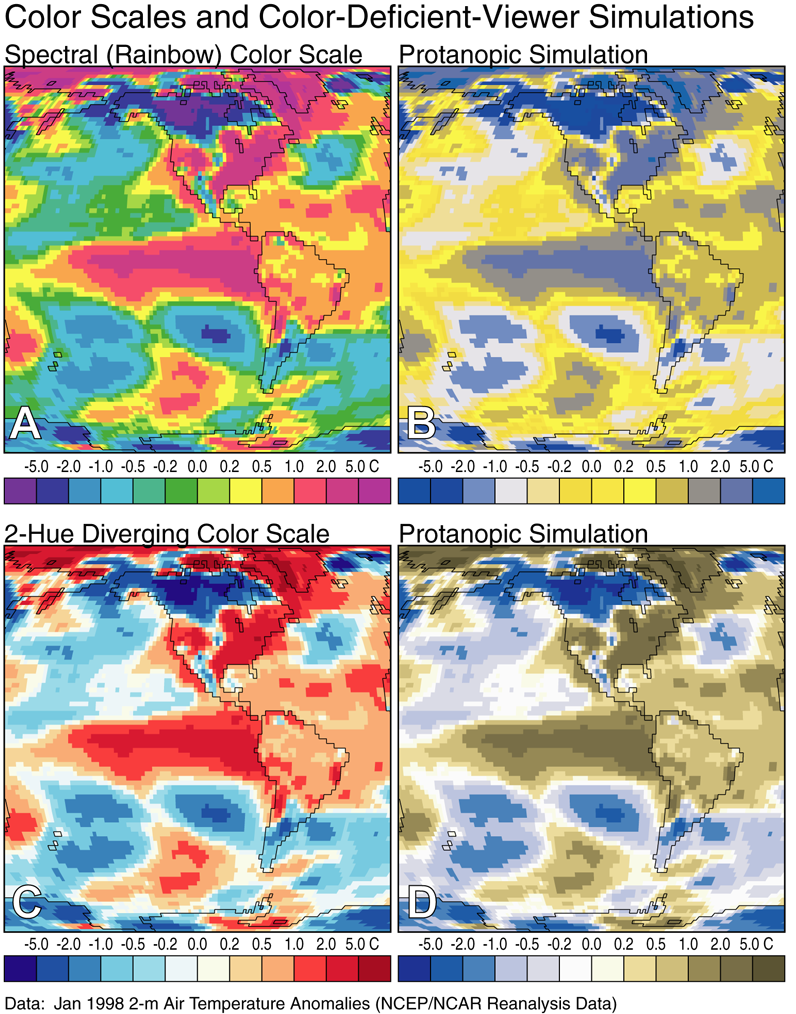
\includegraphics[width=\columnwidth]{lb_fig1.png}
\caption{ \label{color_scales}
    This is Figure 1 from \citep{light2004end}. 
    }
\end{center}
\end{figure}

Good figures are hard to make, there's no question about it.
That goes double for deciding which figures to include in your space-limited abstract.

When you make the decision to create a color figure, take some time to think about the colors that you use.
We think that \citep{light2004end, borland2007rainbow} make a good case for not using the typical rainbow-spectrum color scheme (e.g. Fig.~\ref{color_scales}).
Don't confuse ``pretty'' with ``meaningful.''

A suggestion by \citep{green2011colour} is that color schemes should be perceived as monotonically increasing when used to display intensity maps of various sorts (such as topography, etc.). 
This generally does not happen with most rainbow color schemes.
A monotonically increasing color scheme also does its job whether printed in color or grayscale.
See Fig.~\ref{SaturationColors}

If you need tables to be the full width of the page, just use their starred versions, like \verb=\begin{table*}= instead of \verb=\begin{table}=. 
However, if you want figures to be the full width and you use the starred version \verb=\begin{figure*}=, then you'll find that the figure is either always at the top of the page or on its own page.
This is a \LaTeX\ limitation.

\begin{figure*}
\begin{center}
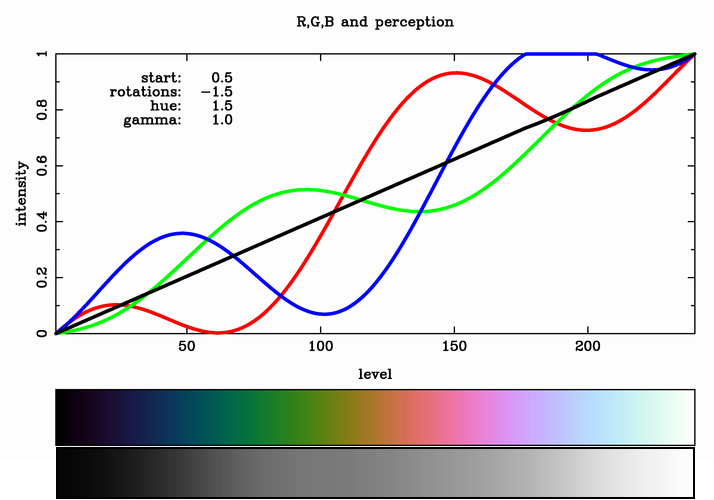
\includegraphics[width=\textwidth]{rgb-grey-morehue.png}
\caption[CubeHelix Color Schemes]{
   \label{SaturationColors}
    Modified from \url{https://www.mrao.cam.ac.uk/~dag/CUBEHELIX}. 
    The color and greyscale bars are both increasining in brightness monotonically.
    }
\end{center}
\end{figure*}

\subsection*{\hspace{0.5cm}Copyright Information:}

This work is licensed under the Creative Commons Attribution-Noncommercial-Share Alike 3.0 License.
To view a copy of this license, visit \url{http://creativecommons.org/licenses/by-nc-sa/3.0/}; or, (b) send a letter to Creative Commons, 171 2nd Street, Suite 300, San Francisco, California, 94105, USA.

Does this mean that if you write an abstract using this template that you are required by law to credit us and to release the paper under the same kind of Creative Commons license?
No, it doesn't.
Mostly for the same reasons that you don't credit the authors of \LaTeX\ when using their software to create documents.
What it does do is allow anyone, even the LPI Meeting Staff, to take a copy of this template and modify it (or not), and place it on their web pages for folks
to use.

Why not just dedicate it to the public domain, you might ask?
Well, we did spend some time on it and would like to be recognized.
Using the Creative Commons license above allows us to retain copyright, request that derivative templates credit us, but also allow for \emph{anyone} to make derivative works, in addition to a few other rights and restrictions.
If you want to know more, visit the Creative Commons web site.
You may even want to check out the Science Commons at \url{http://science.creativecommons.org/}.


\subsection*{Works that you reference}
Note that you will not use a \verb=\subsection= heading to start this section, that's taken care of for you.
Using \texttt{bibtex} with the \texttt{inparaenum} option and the included LPSC bibliographystyle approximates the reference-style that has emerged for LPSC abstracts.

%\begin{flushleft}
\begin{inparaenum}
  \bibliographystyle{lpsc}
  \fussy
  \raggedright
  \bibliography{templatebibliography}
\end{inparaenum}
%\end{flushleft}



\end{document}

